% Journal:
%   Journal of Ambient Intelligence and Smart Environments (JAISE), IOS Press
%   Web Intelligence and Agent Systems: An International Journal (wias)
%   Semantic Web: Interoperability, Usability, Applicability (SW)
% Latex 2e
% Test file iosart2c.tex

%[seceqn,secfloat,secthm,crcready]

% options: wias, jaise, sw
\documentclass{iosart2c}

\usepackage[T1]{fontenc}
\usepackage{times}%
\usepackage{listings}
\usepackage{tabularx}
%\usepackage{algorithm}
\usepackage{pdflscape}
\usepackage{paralist}
\usepackage[hidelinks]{hyperref}
\usepackage{url}
\usepackage{natbib}% for bibliography sorting/compressing
\usepackage{amsmath}
\usepackage{amssymb}
%\usepackage{endnotes}
\usepackage{floatrow}
\usepackage{bbding}
\usepackage{graphics}
\usepackage{graphicx}
\usepackage{epstopdf}
\usepackage{xcolor}
\usepackage{epsfig,color,subfigure}
%\usepackage{tikz}
%\usepackage{tikzscale}
\usepackage{pgf-pie}
\usepackage{pgfplots}
\usepackage{soul}
\pgfplotsset{compat=1.5}
%\usetikzlibrary{backgrounds}
%\usepackage[scaled=0.87]{helvet}
\usepackage{textcomp}
\usepackage{enumitem}
\usepackage{colortbl}   % Provides \rowcolor
\usepackage{calc}       % For doing math with dimensions
\usepackage{setspace}
\usepgfplotslibrary{dateplot}
%\usetikzlibrary{shapes.geometric, arrows}
\usetikzlibrary{shapes,decorations,arrows}
\usetikzlibrary{positioning}
\usetikzlibrary{calc}

%\usepackage{bibentry}


\newcommand{\figfontsize}{\footnotesize}

%%%%%%%%%%% Put your definitions here
\newcommand{\TODO}[1]{\textcolor{red}{\textbf{[TODO:#1]}}}
\newcommand{\maria}[1]{\textcolor{blue}{\textbf{[MARIA:#1]}}}
\newcommand{\py}[1]{\textcolor{olive}{\textbf{[PIERRE-YVES TO:#1]}}}
\newcommand{\ghis}[1]{\textcolor{brown}{\textbf{[GHIS TO:#1]}}}
\newcommand{\js}[1]{\textcolor{brown}{\textbf{[JS:#1]}}}

% Language Definitions for Turtle
\definecolor{MyLightGray}{RGB}{200, 200,200}
\lstdefinelanguage{turtle}
{
    columns=fullflexible,
    keywordstyle=\color{red},
    morekeywords={PREFIX,SELECT,DISTINCT,UNION,FILTER,ORDER,BY,REGEX,STR,STRSTARTS,GRAPH,isBlank},
    morecomment=[l]{\#},
    tabsize=4,
    frame=lines,
    numbers=left,
    numberfirstline=true,
    xleftmargin=2.5em,
    framexleftmargin=2.8em,
    stepnumber=1,    
    firstnumber=1,
    alsoletter={-?}, % allowed in names
    morecomment=[s][\color{blue}]{<}{>},
    commentstyle=\color{green!40!black},
    basicstyle=\scriptsize\ttfamily\color{black},
    %numberstyle=\color{black},
    morestring=[b][\color{black}]\",
    backgroundcolor=\color{background},    
    showstringspaces=false
}

%% language json
\colorlet{punct}{red!60!black}
\definecolor{background}{HTML}{EEEEEE}
\definecolor{delim}{RGB}{20,105,176}
\colorlet{numb}{magenta!60!black}

\lstdefinelanguage{json}{
    basicstyle=\scriptsize\ttfamily,
    stepnumber=1,
    numbersep=8pt,
    showstringspaces=false,
    breaklines=true,
    numbers=left,
    numberfirstline=true,
    frame=lines,
    backgroundcolor=\color{background},
    literate=
     *{0}{{{\color{numb}0}}}{1}
      {1}{{{\color{numb}1}}}{1}
      {2}{{{\color{numb}2}}}{1}
      {3}{{{\color{numb}3}}}{1}
      {4}{{{\color{numb}4}}}{1}
      {5}{{{\color{numb}5}}}{1}
      {6}{{{\color{numb}6}}}{1}
      {7}{{{\color{numb}7}}}{1}
      {8}{{{\color{numb}8}}}{1}
      {9}{{{\color{numb}9}}}{1}
      {:}{{{\color{punct}{:}}}}{1}
      {,}{{{\color{punct}{,}}}}{1}
      {\{}{{{\color{delim}{\{}}}}{1}
      {\}}{{{\color{delim}{\}}}}}{1}
      {[}{{{\color{delim}{[}}}}{1}
      {]}{{{\color{delim}{]}}}}{1},
}
%%%%%%%%%%% End of definitions

\newcolumntype{d}[1]{D{.}{.}{#1}}


\firstpage{1} \lastpage{5} \volume{1} \pubyear{2014}


\begin{document}

\begin{frontmatter}                        % The preamble begins here.

%
%\pretitle{Pretitle}
\title{Linked Open Vocabularies (LOV): a gateway to reusable semantic vocabularies on the Web}

%\thanks{Footnote in title.}

\runningtitle{LOV: a gateway to reusable semantic vocabularies on the Web}
%\subtitle{Subtitle}

\review{Name Surname, University, Country}{Name Surname, University, Country}{Name Surname, University, Country}


\author[A]{\fnms{Pierre-Yves} \snm{Vandenbussche}\thanks{Thanks to Am\'elie Gyrard, Thomas Francart, Th\'er\`{e}ze Rogez, Laurent Irles and Anthony McCauley for their help on the project.}},
\author[B]{\fnms{Ghislain A.} \snm{Atemezing}},
\author[C]{\fnms{Mar\'ia} \snm{Poveda-Villal\'on}}
and
\author[D]{\fnms{Bernard} \snm{Vatant}}
\runningauthor{Pierre-Yves V. et al.}
\address[A]{Fujitsu (Ireland) Limited, Swords, Co. Dublin, Ireland\\
E-mail: pierre-yves.vandenbussche@ie.fujitsu.com}
\address[B]{Mondeca, 35 boulevard de Strasbourg, 75010 Paris, France\\
E-mail: ghislain.atemezing@mondeca.com}
\address[C]{Ontology Engineering Group (OEG), 
Universidad Polit\'ecnica de Madrid, Madrid, Spain\\
E-mail: mpoveda@fi.upm.es}
\address[D]{Mondeca, 35 boulevard de Strasbourg, 75010 Paris, France
\\
E-mail: bernard.vatant@mondeca.com}


%%% Abstract%%%%%%
%%%%%%%%%%%%%%%%%%

\begin{abstract}

One of the major barriers to the deployment of 
Linked Data is the difficulty that data publishers have in determining which vocabularies to use to describe the semantics of data. This systematic report describes Linked Open Vocabularies (LOV), a high-quality catalogue of reusable vocabularies for the description of data on the Web. The LOV initiative gathers and makes visible indicators such as the interconnections between vocabularies and each vocabulary's version history, along with past and current editor (individual or organization). The report details the various components of the system along with some innovations, such as the introduction of a property-level boost in the vocabulary search scoring that takes into account the property's type (e.g, \texttt{dc:comment}) associated with a matching literal value. By providing an extensive range of data access methods (full-text search, SPARQL endpoint, API, data dump or UI), the project aims at facilitating the reuse of well-documented vocabularies in the Linked Data ecosystem. The adoption of LOV by many applications and methods shows the importance of such a set of vocabularies and related features for ontology design and the publication of data on the Web.

\end{abstract}

\begin{keyword}
LOV\sep Linked Open Vocabularies\sep Ontology search\sep Linked Data\sep Vocabulary catalogue
%\sep keyword five
\end{keyword}

\end{frontmatter}


%%%% Section: INTRO %%%%
%%%%%%%%%%%%%%%%%%%%%%%%
\section{Introduction}
The last two decades have seen the emergence of a ``Semantic Web'' enabling humans and computer systems to exchange data with unambiguous, shared meaning. This vision has been supported by World Wide Web Consortium (W3C) Recommendations such as the Resource Description Framework (RDF), RDF-Schema and the Web Ontology Language (OWL). Thanks to a major effort in publishing data following Semantic Web and Linked Data principles~\cite{timld}, there are now tens of billions of facts spanning hundreds of linked datasets on the Web covering a wide range of topics.
Access to the data is facilitated by portals (such as Datahub\footnote{\url{http://datahub.io/}} or UK Government Data\footnote{\url{http://data.gov.uk/}}) or direct publication by organisations (e.g. New York Times\footnote{\url{http://data.nytimes.com/}}). 

Despite the enormous volume of data now available on the Web, the Linked Data community has relatively little interest in vocabulary\footnote{We use the terms ``semantic vocabulary'', ``vocabulary'' and ``ontology'' interchangeably.} management, focusing rather on the data itself. A vocabulary consists of classes, properties and datatypes that define the meaning of data. RDF vocabularies are themselves expressed and published following the Linked Data principles; this gives humans and machines access to the definitions of the terms used to qualify the data. Unfortunately some vocabularies are not published or are no longer not available; this breaks the semantic interoperability of the data, one of the fundamental principles of the Semantic Web~\cite{janowicz2014five}.

The Linked Open Vocabularies (LOV) initiative\footnote{\url{http://lov.okfn.org/dataset/lov/}} is an innovative observatory of the semantic vocabularies ecosystem. Started in March 2011, as part of the DataLift research project~\cite{scharffe_2012} and hosted by the Open Knowledge Foundation, LOV gathers and makes visible  indicators not previously harvested, such as the interconnections between vocabularies, the versioning history along with past and current editor  (individual or organization). The number of vocabularies indexed by LOV is constantly growing (527 as of October 2015) thanks to a community effort. It is the only catalogue, to the best of our knowledge, that accepts all types of search criteria: metadata search, ontology search, APIs, a comprehensive dump file and SPARQL endpoint access. 

The purpose of LOV is to promote and facilitate the reuse of well documented vocabularies in the Linked Data ecosystem. In D'Aquin and Noy~\cite{AquinJoWS12}'s categorisation of ontology libraries, LOV falls into the categories \textit{``curated ontology directory''}  and \textit{``application platform''}. Specifically, LOV supports the following main activities for the design of ontologies and the publication of data on the Web~\cite{MC10, ohdeploying, pedrinaci2014, villata2012}:

\begin{description}
 \item [Ontology Search.] LOV enables searching for vocabulary terms (class, property, datatype) based on domain: vocabularies (and therefore vocabulary terms) are categorised according to the domain they address.
 \item [Ontology Assessment.] LOV provides a ranking (cf. Section \ref{sssec:search} for each term retrieved by a keyword search to assist in ontology assessment.
 \item [Ontology Mapping.] LOV categorizes seven different types of relationships between ontologies: metadata, import, specialization, generalization, extension and equivalence (cf. Section \ref{sec:vocabLevelAnalysis}). These relationships can be useful for finding alignments between ontologies. 
\end{description}

This report is structured as follows: in the next section, we provide statistics on the usage of LOV. In Section~\ref{sec:arch}, we describe the components and features of the system. Thereafter, in Section~\ref{sec:lovecosystem}, we provide an overview of some applications and research projects based on and motivated by the LOV system. In Section~\ref{sec:related}, we report on related work. The limitations and further development of LOV are discussed in Section~\ref{sec:discussion}. We conclude in Section~\ref{sec:conclusion}.


%%%%%LOV state%%%%%%%
%%%%%%%%%%%%%%%%%%%%%
\section{LOV state}\label{sec:state}

The LOV dataset consists of 527 vocabularies as of October 2015\footnote{However, the figures and evaluation used in this report are based on LOV catalogue with 511 vocabularies as of June 2015.}. Figure \ref{fig:evolLOV} shows the evolution of the number of vocabularies inserted in the LOV dataset since March 2011. The addition of new vocabularies to LOV has been fairly constant with two exceptions: 
\begin{inparaenum}[1)] 
	\item the deployment of LOV version 2 [early 2012] automated most of the vocabulary analyses, resulting in the increase number of vocabularies ; and
	\item the deployment of LOV version 3 [early 2015], resulting in a small decrease and plateau of the vocabularies. At that time we were considering removing offline vocabularies but finally decided to keep them with a special flag, making LOV the only source of continuity for datasets referencing unreachable vocabularies.
		
	
	
\end{inparaenum} 


\begin{figure}[htb]
   \resizebox{1.04\linewidth}{!}{\begin{tikzpicture}
\begin{axis}[
axis on top,
legend style={at={(0.02,0.98)},anchor=north west,opacity=0.8, font=\scriptsize},
date coordinates in=x,
xticklabel={\year-\month},
x tick label style={align=right,rotate=65,font=\scriptsize},
date ZERO=2012-04-01, % Set near lowest date
xmin={2011-02-01}, % A date with no time is assumed to have a time of 00:00
xmax={2014-12-31},
ymin={0},
xtick={% Set tick marks
2011-04-01,
2011-07-01,
2011-10-01,
2012-01-01,
2012-04-01,
2012-07-01,
2012-10-01, 
2013-01-01,
2013-04-01,
2013-07-01,
2013-10-01,
2014-01-01,
2014-04-01,
2014-07-01,
2014-10-01,
2015-01-01},
grid=major,
stack plots=y,
area style,
]


\pgfplotstableread{PGFPlots/LOVSizeEvol.dat}\thisTable

\addplot+[black,fill=orange] table[x=date,y=nbVocabs]{\thisTable}\closedcycle;
\addlegendentry{Vocab Number}






%\addplot table[x=date,y=nbClasses]{\thisTable};


%\addplot table[x=date,y=nbProperties]{\thisTable};


\end{axis}
\end{tikzpicture}}
   \caption{\label{fig:evolLOV} Evolution of the number of vocabularies in LOV from March 2011 to June 2015.
   }
\end{figure}


By observing the vocabularies contained in LOV as a whole, we can extract some information about Semantic Web adoption and dynamics. Figure~\ref{fig:creaevol} shows the distribution of LOV vocabularies by creation date. The distribution follows a bell curve with its peak in 2011. It is worth noting that a decrease in number of vocabulary creation does not necessarily mean a decrease in use of the technology but rather that the existing vocabularies now cover a large part of the semantic description needed. When looking at the last modified date of the same vocabularies (as illustrated in Figure~\ref{fig:modifevol}), we see that LOV vocabularies are part of a living ecosystem in constant evolution. 

\begin{figure}[htb]
\resizebox{\linewidth}{!}{\makeatletter
\long\def\ifnodedefined#1#2#3{%
    \@ifundefined{pgf@sh@ns@#1}{#3}{#2}%
}
\makeatother

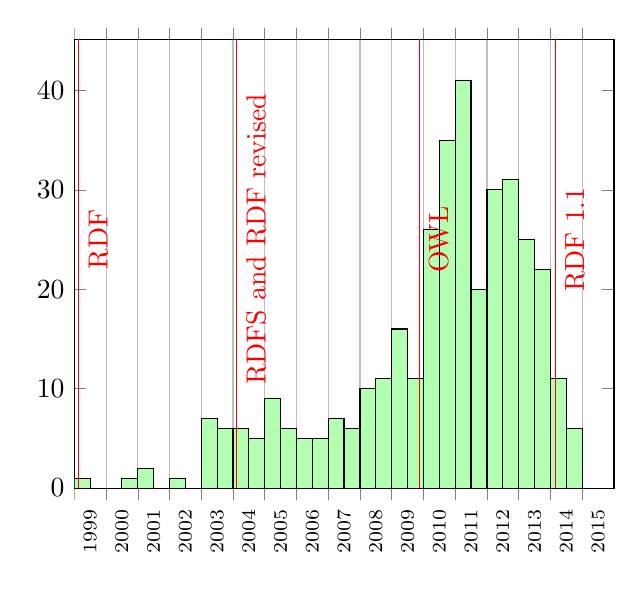
\begin{tikzpicture}
\begin{axis}[
date coordinates in=x,
x tick label style={align=left,rotate=90,font=\scriptsize},
date ZERO=1998-01-01,% <- improves precision!
xmin={1998-01-01}, % A date with no time is assumed to have a time of 00:00
xmax={2015-01-01},
ybar interval,
ymin={0},
  xticklabel={\year},
xtick={% Set tick marks CAREFUL the year has been decremented by one year ... was not able to figure out how to do that properly...
1998-01-01,
1999-01-01,
2000-01-01,
2001-01-01,
2002-01-01,
2003-01-01,
2004-01-01,
2005-01-01,
2006-01-01,
2007-01-01,
2008-01-01,
2009-01-01,
2010-01-01,
2011-01-01,
2012-01-01,
2013-01-01,
2014-01-01,
2015-01-01
},
]
\addplot[fill=green!30!white] coordinates {
(1998-01-01,1)
(1998-07-01,0)
(1999-01-01,0)
(1999-07-01,1)
(2000-01-01,2)
(2000-07-01,0)
(2001-01-01,1)
(2001-07-01,0)
(2002-01-01,7)
(2002-07-01,6)
(2003-01-01,6)
(2003-07-01,5)
(2004-01-01,9)
(2004-07-01,6)
(2005-01-01,5)
(2005-07-01,5)
(2006-01-01,7)
(2006-07-01,6)
(2007-01-01,10)
(2007-07-01,11)
(2008-01-01,16)
(2008-07-01,11)
(2009-01-01,26)
(2009-07-01,35)
(2010-01-01,41)
(2010-07-01,20)
(2011-01-01,30)
(2011-07-01,31)
(2012-01-01,25)
(2012-07-01,22)
(2013-01-01,11)
(2013-07-01,6)
(2014-01-01,0)
(2014-07-01,0)
};
\addplot[red,sharp plot,update limits=false] 
	coordinates {(1998-02-22,0) (1998-02-22,50)} 
	node[below, rotate=90] at (axis cs:1998-02-22,25) {RDF};
\addplot[red,sharp plot,update limits=false] 
	coordinates {(2013-02-25,0) (2013-02-25,50)} 
	node[below, rotate=90] at (axis cs:2013-02-25,25) {RDF 1.1};
\addplot[red,sharp plot,update limits=false] 
	coordinates {(2003-02-10,0) (2003-02-10,50)} 
	node[below, rotate=90] at (axis cs:2003-02-10,25) {RDFS and RDF revised};
\addplot[red,sharp plot,update limits=false] 
	coordinates {(2008-11-15,0) (2008-11-15,50)} 
	node[below, rotate=90] at (axis cs:2008-11-15,25) {OWL};
\end{axis}
\end{tikzpicture}}
\caption{\label{fig:creaevol} Distribution of LOV vocabularies by creation date. For indication, we use vertical red lines to mark the official release dates of the main Semantic Web languages (RDF, RDFS and OWL).}
\end{figure}

\begin{figure}[htb]
\resizebox{\linewidth}{!}{\makeatletter
\long\def\ifnodedefined#1#2#3{%
    \@ifundefined{pgf@sh@ns@#1}{#3}{#2}%
}
\makeatother

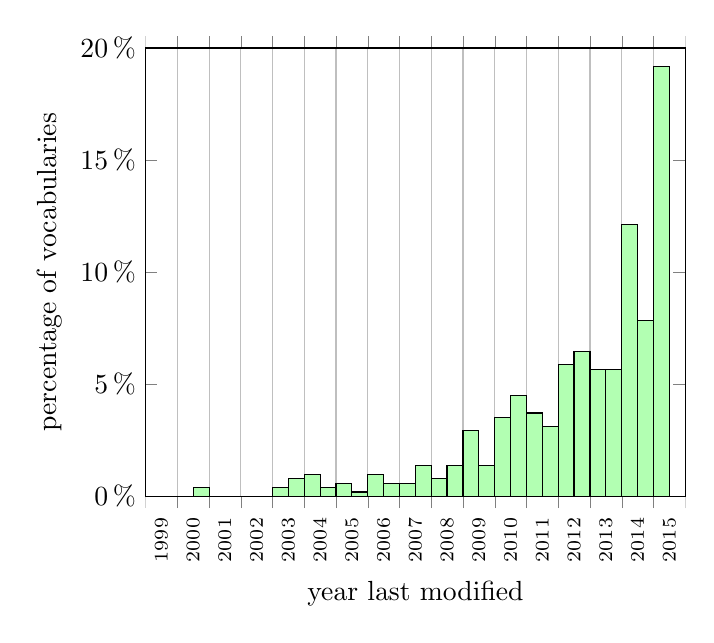
\begin{tikzpicture}
\begin{axis}[
    ylabel=percentage of vocabularies,
    xlabel=year last modified,
date coordinates in=x,
x tick label style={align=left,rotate=90,font=\scriptsize},
date ZERO=1998-01-01,% <- improves precision!
xmin={1998-01-01}, % A date with no time is assumed to have a time of 00:00
xmax={2015-01-01},
ybar interval,
ymin={0},
ymax={20},
yticklabel=\pgfmathprintnumber{\tick}\,$\%$,
  xticklabel={\year},
xtick={% Set tick marks CAREFUL the year has been decremented by one year ... was not able to figure out how to do that properly...
1998-01-01,
1999-01-01,
2000-01-01,
2001-01-01,
2002-01-01,
2003-01-01,
2004-01-01,
2005-01-01,
2006-01-01,
2007-01-01,
2008-01-01,
2009-01-01,
2010-01-01,
2011-01-01,
2012-01-01,
2013-01-01,
2014-01-01,
2015-01-01
},
]
\addplot[fill=green!30!white] coordinates {
(1998-01-01,0)
(1998-07-01,0)
(1999-01-01,0)
(1999-07-01,0.391)
(2000-01-01,0)
(2000-07-01,0)
(2001-01-01,0)
(2001-07-01,0)
(2002-01-01,0.391)
(2002-07-01,0.783)
(2003-01-01,0.978)
(2003-07-01,0.391)
(2004-01-01,0.587)
(2004-07-01,0.196)
(2005-01-01,0.978)
(2005-07-01,0.587)
(2006-01-01,0.587)
(2006-07-01,1.370)
(2007-01-01,0.783)
(2007-07-01,1.370)
(2008-01-01,2.935)
(2008-07-01,1.370)
(2009-01-01,3.523)
(2009-07-01,4.501)
(2010-01-01,3.718)
(2010-07-01,3.131)
(2011-01-01,5.871)
(2011-07-01,6.458)
(2012-01-01,5.675)
(2012-07-01,5.675)
(2013-01-01,12.133)
(2013-07-01,7.828)
(2014-01-01,19.178)
(2014-07-01,0)
};
\end{axis}
\end{tikzpicture}}
\caption{\label{fig:modifevol} Distribution of LOV vocabularies by last modified date.}
\end{figure}

 
Overall, the LOV dataset contains 20,000 classes and almost 30,000 properties. The median is 9 classes and 17 properties per vocabulary. Table \ref{tab:elements} presents a breakdown of LOV content by vocabulary element type. In this Table, the  \emph{Classes} type refers to any instance of {\small\texttt{rdfs:Class}} or {\small\texttt{owl:Class}}; the  \emph{Properties} type refers to any instance of {\small\texttt{rdf:Property}} or by inference, any instance of subclasses of {\small\texttt{rdf:Property}} defined in the OWL language; the \emph{Datatypes} type refers to any instance of {\small\texttt{rdfs:Datatype}}; and finally, the members of a vocabulary class are known as \emph{instances} of the class.

\begin{table}[htb]
\caption{LOV vocabulary element types statistics.}
\begin{tabular}{lrr}
\hline
\textbf{Type} & \textbf{Count} &  \textbf{Median per vocab} \\ \hline
Properties & 29,925 & 17 \\
Classes & 20,034 & 9 \\
Instances & 5,232 & 0 \\
Datatypes & 101 & 0 \\
\hline  
\end{tabular}
\label{tab:elements}
\end{table}

Out of 511 vocabularies, 66.14\% explicitly use the English language for labels/comments, i.e containing \texttt{@en} tag. Table \ref{tab:language} presents the number and percentage of vocabularies using the top five languages detected in LOV. Figure \ref{fig:langdist} shows the distribution of vocabularies per number of languages explicitly 
used: 27.98\% of the vocabularies still do not provide any language information, and only 14.68\% of the vocabularies are multilingual. In total, 45 languages are used by vocabularies in LOV. We will discuss the importance of providing multilingual vocabularies in Section \ref{sec:conclusion}.

 \begin{table}[h!tb]
\caption{Top five languages detected in the LOV catalogue, showing numbers and percentages of vocabularies using them. A vocabulary can make use of multiple languages.}
\begin{tabular}{lrr}
\hline
\textbf{Language} & \textbf{\# vocabs} & \textbf{\% vocabs (out of 511)}  \\ \hline
English & 338 & 66.14\%      \\
French & 37 & 7.24\%      \\
Spanish & 25 & 4.89\%      \\
German & 19 & 3.72\%      \\
Italian & 18 & 3.52\%      \\
\hline  
\end{tabular}
\label{tab:language}
\end{table}


From January to June 2015, more than 1.4 million searches were conducted on LOV\footnote{This figure includes searches from the API and UI as well as searches with and without keywords such as ``all agents that participated in vocabulary design and publication in the geo-location domain''.}. A breakdown of searches per element type is provided in Table \ref{tab:searchcategory}. We can see that agent search (for person or organisation) is the most prevalent; this is a new feature in LOV version 3. This might be explained by the uniqueness (when compared to other ontology catalogues) and the recent development of this feature in LOV, which now allows a user to visualise who defined or published vocabularies. Searches that include keywords (and not only filters) are mainly seek vocabulary terms. Table \ref{tab:toptermsearch} presents the top 10 searched terms between January and June 2015. Although most of the searches are performed through the user interface, an application ecosystem using LOV APIs has surfaced, as shown in Figure \ref{fig:apivsui}. 

\begin{figure}[htb]
\resizebox{\linewidth}{!}{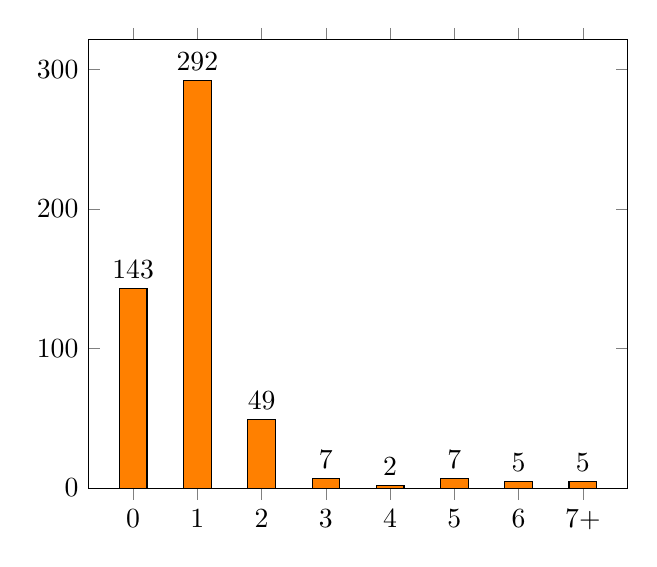
\begin{tikzpicture}
\begin{axis}[
    ybar,
    ymin={0},
    % ylabel={\#vocabularies},
    symbolic x coords={0,1,2,3,4,5,6,7+},
    xtick=data,
    nodes near coords,
    nodes near coords align={vertical},
    ]
\addplot[fill=orange] coordinates {(0,143)
(1,292)
(2,49)
(3,7)
(4,2)
(5,7)
(6,5)
(7+,5)
};
\end{axis}
\end{tikzpicture}}
\caption{\label{fig:langdist} Distribution of LOV vocabularies by number of languages explicitly mentioned using language tag. ``Zero" means that there is no explicit language tag declared (i.e. no literal value of the vocabulary has a language tag).}
\end{figure}


\begin{table*}[h!tb]
\caption{Type of elements searched from January to June 2015 by users in LOV for all searches and those with keyword.}
\begin{tabular}{l|rr|rr}
\hline
\textbf{Element Type } & \textbf{\# searches} & \textbf{\% searches} & \textbf{\# searches} & \textbf{\% searches} \\
 &  & & with keyword & with keyword \\ \hline
Term & 205,682 & 14.19\% & 80,728 & 92.84\% \\
Vocabulary & 178,837 & 12.34\% & 5,918 & 6.81\% \\
Agent & 1,064,597 & 73.47\% & 306 & 0.35\% \\
\hline  
\end{tabular}
\label{tab:searchcategory}
\end{table*}

 \begin{table}[h!tb]
\caption{Top 10 terms searched from January to June 2015 by users in LOV.}
\begin{tabular}{lrr}
\hline
\textbf{Vocabulary Term} & \textbf{\# searches} & \textbf{\% searches} \\ \hline
set & 7,092 & 8.79\% \\
domain & 2,518 & 3.12\% \\
some & 2,473 & 3.06\% \\
status & 1,486 & 1.84\% \\
iso 639 & 1,389 & 1.72\% \\
same & 1,285 & 1.59\% \\
state & 1,235 & 1.53\% \\
supports & 1,145 & 1.42\% \\
start & 887 & 1.1\% \\
space & 864 & 1.07\% \\
\hline  
\end{tabular}
\label{tab:toptermsearch}
\end{table}

\begin{figure}[tb]
	\ffigbox{
		\figfontsize
		\resizebox{\linewidth}{!}{%\documentclass{standalone}
%\usepackage{pgfplots}
%\begin{document}
\begin{tikzpicture}
\begin{semilogyaxis}[
 cycle list name=exotic,
 ylabel=searches number,
 xlabel=month,
% legend pos=outer north east,
 legend style={at={(0.02,0.98)},anchor=north west},
 legend columns=1,
 ymin=0,ymax=500000,
 mark size=2pt,
 xtick={Jan-15,Feb-15,Mar-15,Apr-15,May-15,Jun-15},
 symbolic x coords={Jan-15,Feb-15,Mar-15,Apr-15,May-15,Jun-15},
 xmin=Jan-15,xmax=Jun-15,
 x tick label style={rotate=65,anchor=east,font=\scriptsize}
]
 %colormap={rg}{rgb(0cm)=(1,0,0); rgb(1cm)=(0,1,0)}

\pgfplotstableread{PGFPlots/apiVsui.dat}\thisTable

\addplot table[x=month,y=nbAPI]{\thisTable};
\addlegendentry{API}
\addplot table[x=month,y=nbUI]{\thisTable};
\addlegendentry{UI}

\end{semilogyaxis}
\end{tikzpicture}
%\end{document}}
	}{
	  \caption{\label{fig:apivsui} Evolution of the number of searches through UI and API methods from January to June 2015. Note that the y axis has a logarithmic scale.}
	}
 \end{figure}

Since 2011, the Linked Open Vocabularies initiative has gathered a community of about 480 people interested in various domains, including ontology engineering and data publication. The LOV Google+ community\footnote{\url{https://plus.google.com/communities/108509791366293651606}} is now an important place to discuss, report and announce general facts related to vocabularies on the Web. The LOV dataset itself references 389 resources of type \emph{Person} and 111 of type \emph{Organization} participating in vocabulary design and/or publication.



%%%%%%%%%%%%%%%%%%%%%%%%%%%%%%%%%%%%%%
%%% System components and Features %%%
%%%%%%%%%%%%%%%%%%%%%%%%%%%%%%%%%%%%%%
\section{System Components and Features}\label{sec:arch}
	 The LOV architecture is composed of four main components (cf. Figure~\ref{fig:arch}): 
\begin{inparaenum}[1)] 
	\item \emph{Tracking and Analysis}. Checks for any vocabulary version update and analyses vocabularies' specific features.
	\item \emph{Curation}. Ensures the high quality of the LOV dataset by enabling the community to suggest vocabularies or edit the catalogue.
	\item \emph{Data Access}. Provides access to the data through a large range of methods and protocols to facilitate the use of LOV dataset and
	\item \emph{Data Storage}. Offers a reliable and efficient method for storing and querying the data.
\end{inparaenum} 
Each component provides a set of features detailed in the following subsections.


\begin{figure}[ht!b]
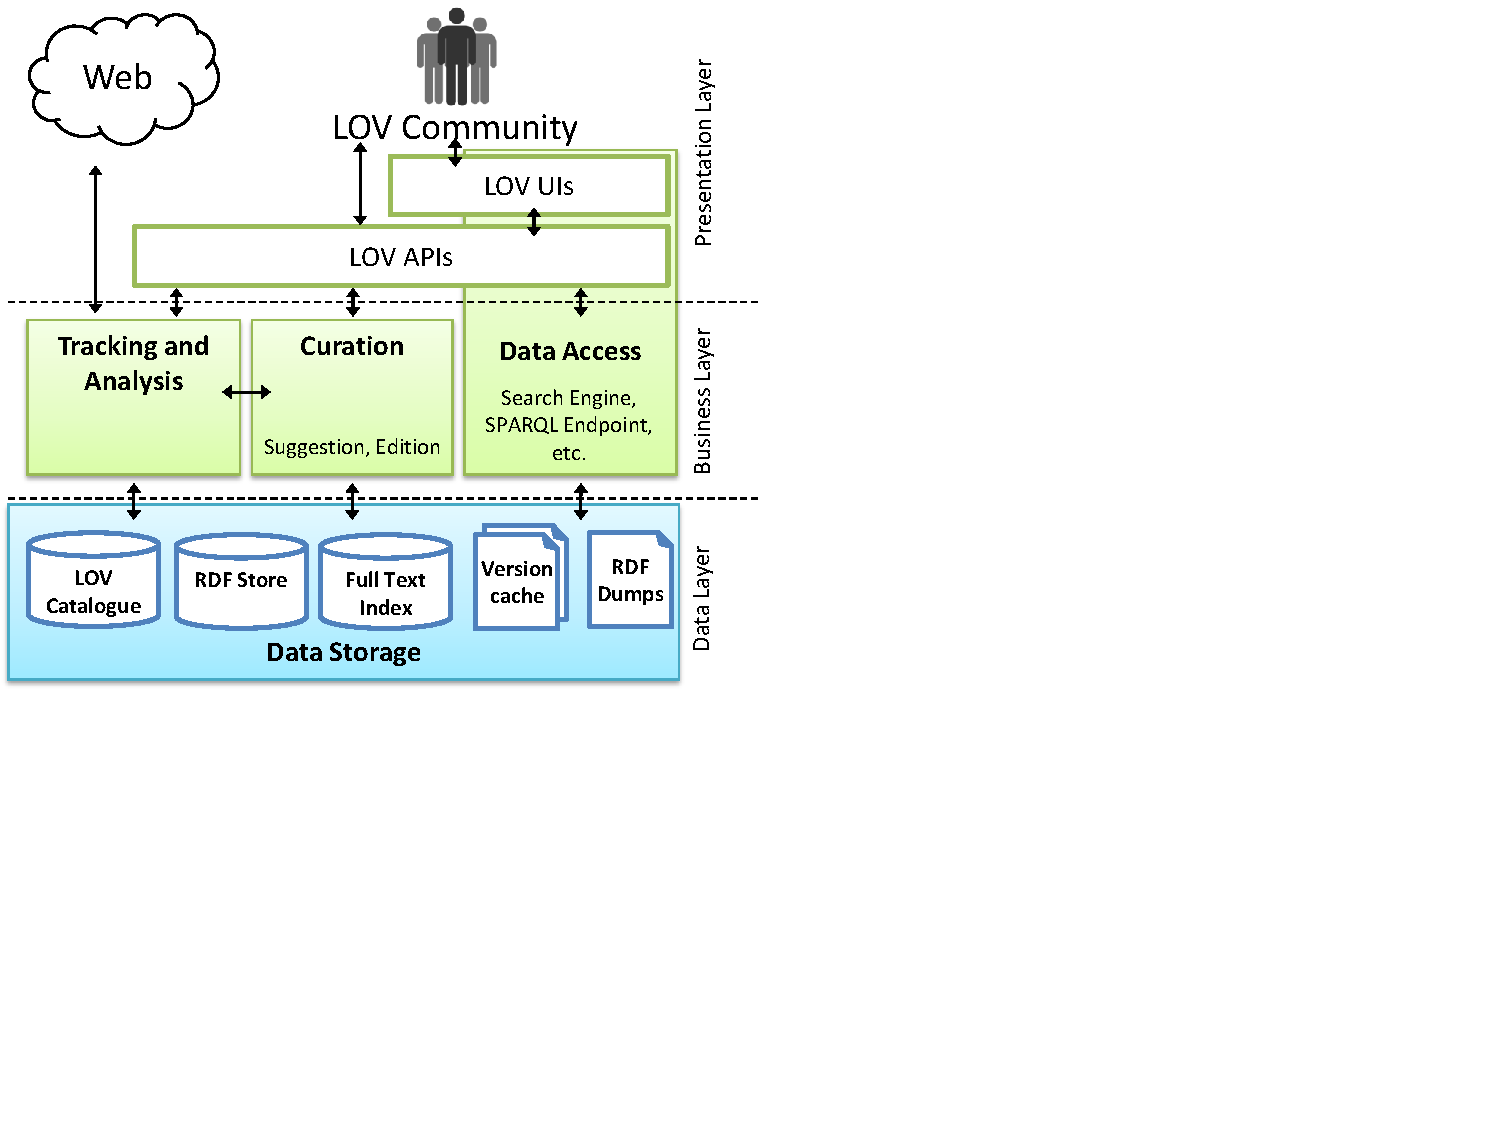
\includegraphics[trim={0cm 7cm 0cm 0cm},scale=.6]{figures/lov_architecture.pdf}
\caption{Overview of the Linked Open Vocabularies Architecture.}
\label{fig:arch}
\end{figure}

\subsection{Tracking and Analysis}
	The \emph{Tracking and Analysis} component dereferences\footnote{A URI is looked up over HTTP to return content in a processable format such as XML/RDF, Notation 3 or Turtle.} LOV vocabularies, stores a version locally (in Notation 3 format) and extracts relevant metadata.

\subsubsection{Vocabulary Level Analysis}\label{sec:vocabLevelAnalysis}
At the vocabulary level, the system extracts three types of information for each vocabulary version (Figure \ref{fig:dcat}):
\begin{itemize}
\item The metadata associated to the vocabulary. This information is explicitly defined within the vocabulary to provide context and useful data about the vocabulary. Some high level vocabularies can be reused for that purpose, such as Dublin Core\footnote{\url{http://purl.org/dc/terms/}} to describe authors, contributors, publishers or Creative Commons\footnote{\url{http://creativecommons.org/ns\#}} for the description of a license.

\item Inlinks/incoming vocabularies, making explicit the \underline{links from} another vocabulary based on the semantic relation of their terms.

\item Outlinks/outgoing vocabularies, making explicit the \underline{links to} another vocabulary based on the semantic relation of their terms.
\end{itemize}

\begin{figure}[ht!b]
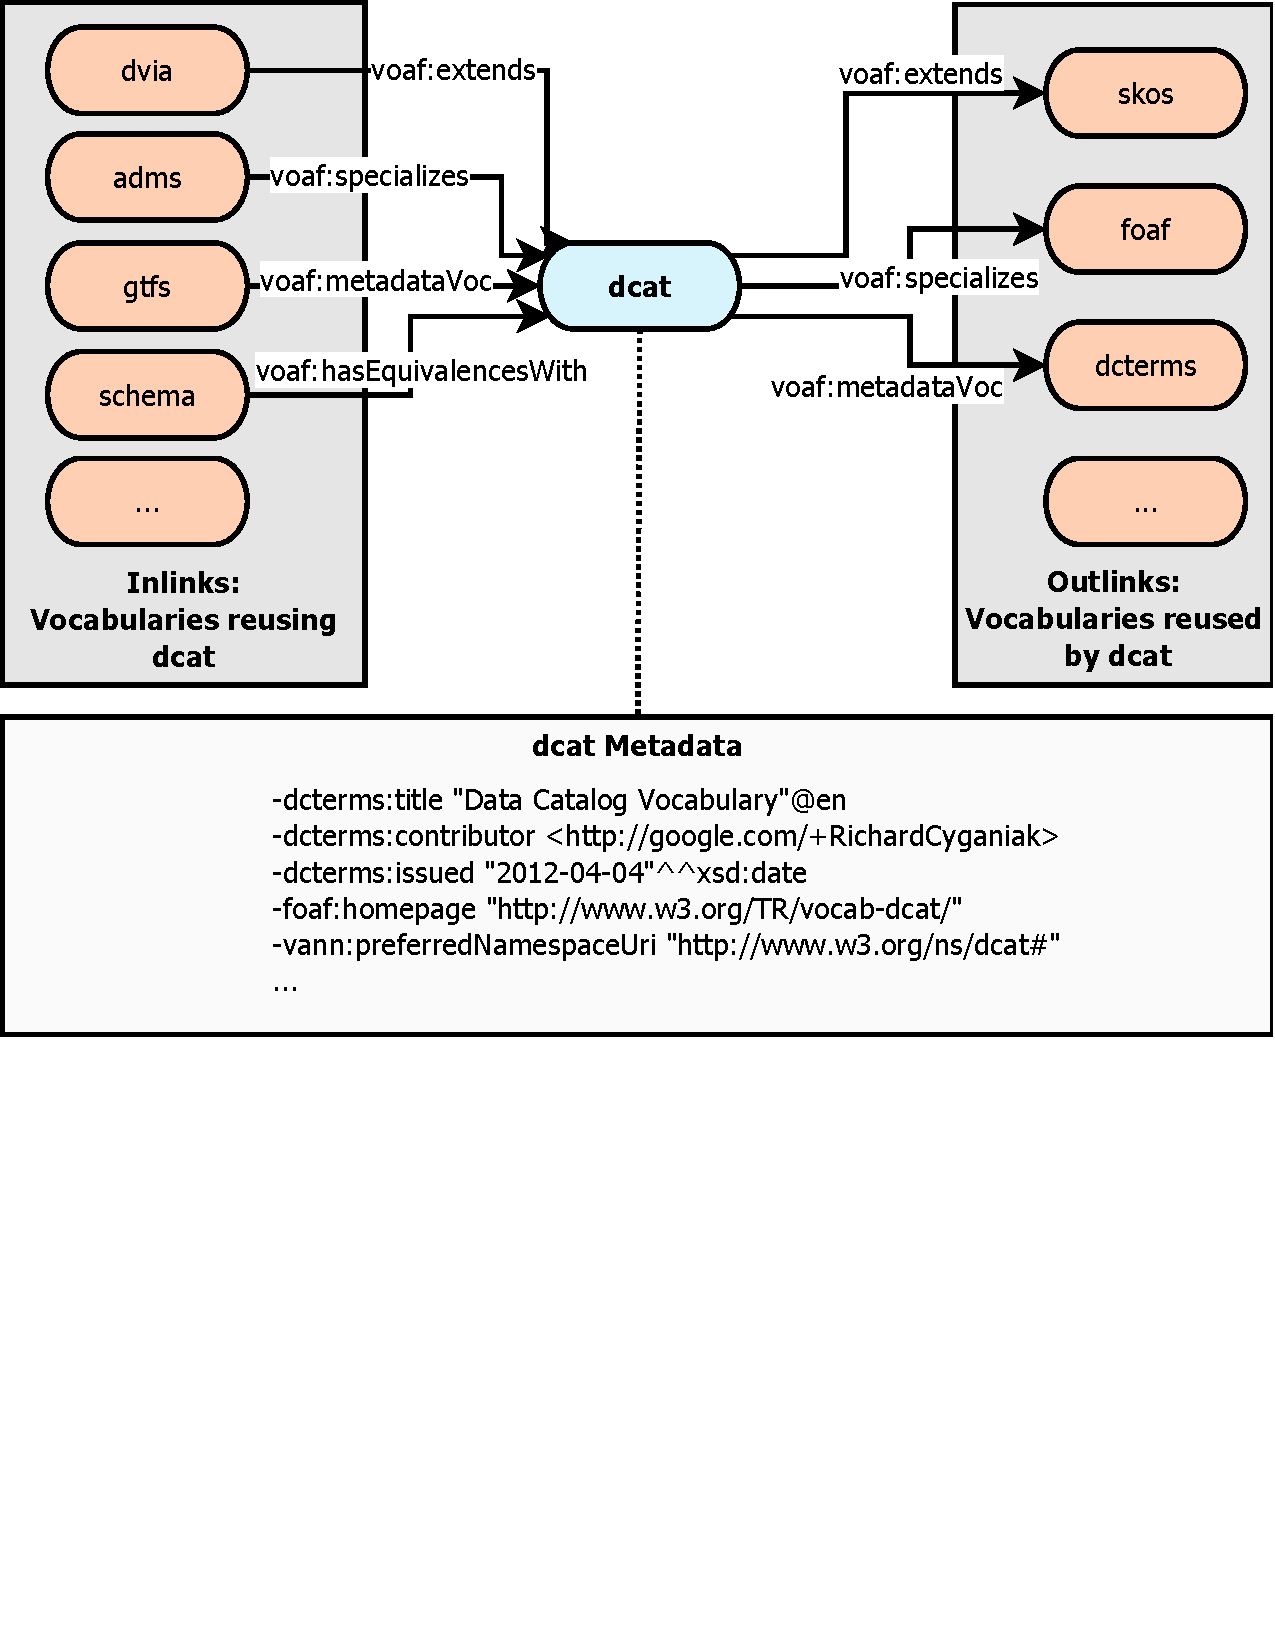
\includegraphics[trim={0cm 10cm 0cm 0cm},width=1\textwidth]{figures/DCAT.pdf}
\caption{Metadata type, vocabulary inlinks and outlinks of DCAT vocabulary.}
\label{fig:dcat}
\end{figure}

Two vocabularies can be interlinked in many different ways. Consider two vocabularies $V1$ and $V2$ such that $V1$ contains a class $c1$ and a property $p1$ and $V2$ contains a class $c2$ and a property $p2$. Relationships between these two vocabularies can be of the following types (the lines and numbers in brackets correspond to real examples presented in Listing \ref{list:voaf}):

		\begin{description}
			\item [Metadata.] some terms from $V2$ are reused to provide metadata about $V1$, Listing \ref{list:voaf} lines 1-2 .

			\item [Import.] some terms from $V2$ are reused with $V1$ to capture the semantic of the data (lines 3 to 4).

			\item [Specialization.] $V1$ defines some subclasses or subproperties (or local restrictions) of $V2$, Listing \ref{list:voaf} lines 5-8.

			\item [Generalization.] $V1$ defines some superclasses or superproperties of $V2$, Listing \ref{list:voaf} lines 9-11.

			\item [Extension.] $V1$ extends the expressivity of $V2$, Listing \ref{list:voaf} lines 12-15.

			\item [Equivalence.] $V1$ declares some equivalent classes or properties with $V2$, Listing \ref{list:voaf} lines 16-20.

			\item [Disjunction.] $V1$ declares some disjunct classes with $V2$, Listing \ref{list:voaf} lines 21-23.
		\end{description}



\begin{lstlisting}[float=*,basicstyle=\tiny,label={list:voaf}, language=turtle, caption={Examples of Inter-vocabulary relationships.}]
# Metadata
<http://www.w3.org/2004/02/skos/core> dct:title "SKOS Vocabulary"@en
# Import - V1 imports V2
<http://purl.org/NET/c4dm/event.owl> owl:imports <http://www.w3.org/2006/time>
# Specialization - c1 is subclass of c2
<http://open.vocab.org/terms/Birth> rdfs:subClassOf <http://purl.org/NET/c4dm/event.owl#Event>
# Specialization - p1 is subproperty of p2  
<http://purl.org/spar/fabio/hasEmbargoDate> rdfs:subPropertyOf <http://purl.org/dc/terms/date>
# Generalization - c1 has for narrower match c2 
<http://semanticweb.cs.vu.nl/2009/11/sem/Place> skos:narrowMatch 
    <http://www.w3.org/2003/01/geo/wgs84_pos#SpatialThing>
# Extension - p1 is inverse of p2
<http://vivoweb.org/ontology/core#translatorOf> owl:inverseOf <http://purl.org/ontology/bibo/translator>
# Extension - p1 has for domain c2
<http://xmlns.com/foaf/0.1/based_near> rdfs:domain <http://www.w3.org/2003/01/geo/wgs84_pos#SpatialThing>
# Equivalence - p1 is equivalent to p2
<http://lsdis.cs.uga.edu/projects/semdis/opus#journal_name> owl:equivalentProperty 
    <http://purl.org/net/nknouf/ns/bibtex#hasJournal>
# Equivalence - c1 is equivalent to c2 
<http://www.loc.gov/mads/rdf/v1#Language> owl:equivalentClass <http://purl.org/dc/terms/LinguisticSystem>
# Disjunction - c1 is disjoint with c2
<http://www.ontologydesignpatterns.org/ont/dul/DUL.owl#TimeInterval>owl:disjointWith 
    <http://www.ontologydesignpatterns.org/ont/dul/ontopic.owl#SubjectSpace>
\end{lstlisting}

These relationships, with the exception of \emph{Import} which is represented by {\small\texttt{owl:imports}}, are captured by the Vocabulary of a Friend\footnote{\url{http://lov.okfn.org/vocommons/voaf/}} (VOAF). Whenever a new vocabulary/vocabulary version is added to LOV, the system automatically detects and adds the inter-vocabulary relationships to the LOV catalogue using specific \emph{Construct} SPARQL queries\footnote{The SPARQL Queries are described in the VOAF vocabulary}. Table \ref{tab:voaf} presents a breakdown of the occurrences of each relation in LOV.

\begin{table}[h!tb]
\caption{Inter-vocabulary relationship types and their number of occurrences in LOV.}
\begin{tabular}{lr}
\hline
\textbf{Inter-vocabulary relationship} & \textbf{\# relations} \\ \hline
voaf:metadataVoc & 2,637 \\
voaf:specializes & 1,269 \\
voaf:extends & 1,031 \\
owl:imports & 373 \\
voaf:hasEquivalencesWith & 201 \\
voaf:generalizes & 57 \\
voaf:hasDisjunctionsWith & 16 \\
\hline  
\end{tabular}
\label{tab:voaf}
\end{table}



\subsubsection{Vocabulary Term Level Analysis}
At the vocabulary term level, the system extracts two types of information:
\begin{itemize}
\item term type (class, property, datatype or instance defined in the namespace of the vocabulary) indexed by the system's search engine so it can be used to filter a search.
\item term natural language annotations (RDF literals) with their predicate and language (e.g. {\small\texttt{rdfs:label}}\\ {\small\texttt{"Temperature"@en}}). This information is provided as is for indexing by the search engine and will later be used (cf. Section \ref{sssec:search}) in the scoring algorithm.
\end{itemize}

The information concerning the usage  of a vocabulary term in Linked Open Data, also called "popularity", is used in LOV search results scoring as explained in Section \ref{sssec:search}. This information is not natively present in the vocabularies and can not be inferred from the LOV dataset. We make use of the LODStats project which gathers comprehensive statistics about RDF datasets~\cite{demter-2012-ekaw}. LOV regularly fetches LODStats raw data\footnote{We retrieve the statistics available at: \url{http://stats.lod2.eu/rdfdocs/void}. Unfortunately this file has been unavailable since June 2014 which explains some differences between the statistics we use and LODStats.} described using the Vocabulary of Interlinked Datasets (VoID)~\cite{void2009} and the Data Cube vocabulary. We pre-process LODStats data before inserting it to LOV. Indeed, there are many duplicates in LODStats representing in fact the same vocabulary URI (e.g., \texttt{foaf} has three different records\footnote{\url{http://stats.lod2.eu/vocabularies?search=foaf}}, and has to be mapped to a single entry in LOV)


\subsection{Curation}
The vocabulary collection is maintained by curators who are responsible for validating metadata information, inserting a vocabulary in the LOV ecosystem, and assigning a review on the suggested vocabulary. 


	\subsubsection{Vocabulary Insertion}\label{sssec:vocabInsert} Compared to other vocabulary catalogues (cf. Section \ref{sec:related}), LOV relies on a semi-automated process for vocabulary insertion. Whereas an automated process focuses only on volume, in our process, we focus on the quality of each vocabulary and therefore the quality of the overall LOV ecosystem. Suggestions come from the community and from inter-vocabulary reference links. Our system provides a feature to suggest\footnote{\url{http://lov.okfn.org/dataset/lov/suggest/}} the insertion of a new vocabulary. This feature allows a user to check what information the LOV system can automatically detect and extract. LOV curators then check whether the vocabulary meets the following LOV quality requirements:
\begin{enumerate}
 \item a vocabulary should be written in RDF and be dereferenceable;
 \item a vocabulary should be parsable without error (warnings are tolerated);
 \item all vocabulary terms (classes, properties and datatypes) in a vocabulary should have an \\ {\small\texttt{rdfs:label}};
 \item a vocabulary should refer to and reuse relevant existing ones; and
 \item a vocabulary should provide some metadata about the vocabulary itself (at least a title).
\end{enumerate}
If a suggested vocabulary meets these criteria it is then inserted in the LOV catalogue. During this process, LOV curators keep the authors informed and help them to improve their vocabulary quality. As a result of our experience in vocabulary publication, we developed a handbook of metadata recommendations for Linked Open Data vocabularies to help in publishing well documented vocabularies~\cite{vandenbussche2011metadata}.


	\subsubsection{Vocabulary Review}
When automatic extraction of metadata fails, LOV curators enhance the description available in the system and notify the vocabulary authors of the pitfalls' report. This manual task usually consists in checking for any additional information present in the HTML documentation (targeted for humans) and not reflected in the RDF description. The documentation provided by the LOV system assists users in understanding the semantics of each vocabulary term and therefore of any data using the term. For instance, information about the creator and publisher is a key indication for a vocabulary user in case help or clarification is required from the author, or to assess the stability of that artifact. About 55\% of the vocabularies specify at least one creator, contributor or editor. We augment this information using manually gathered information, leading to the inclusion of data about the creator in over 85\% of the vocabularies in LOV. The database stores every version of a vocabulary since its first issue. For each version, a user can access the file (particularly useful when the original online file is no longer available). A script automatically checks for vocabulary updates on a daily basis. When a new version is detected, it is stored locally, and the statistics about that vocabulary are recomputed. Similarly we ensure that curated review for each vocabulary is less than one year old by sending curators a notification when a vocabulary review is older than eleven months. In both cases, curators update the vocabulary review accordingly. 



\subsection{Data Access}

The LOV system (code and data) is published under a Creative Commons 4.0 license\footnote{\url{https://creativecommons.org/licenses/by/4.0/}} (CC BY 4.0). Users and applications can access the LOV data in four ways:
		\begin{enumerate} 
			\item Query the LOV search engine to find the most relevant vocabulary terms, vocabularies or agents matching keywords and/or filters;
			\item Download data dumps of the LOV catalogue in RDF Notation 3 format or the LOV catalogue and the latest version of each vocabulary in RDF N-quads format;
			\item Run SPARQL queries on the LOV SPARQL Endpoint; and
			\item Use the LOV API which provides a full access to LOV data for software applications.
		\end{enumerate}
		
	

\subsubsection{Search Engine}\label{sssec:search}
In \cite{butt2014}, Butt \emph{et al.} compare eight different ranking methods grouped in two categories for querying vocabulary terms:
\begin{enumerate}
	\item Content-based Ranking Models: tf-idf, BM25, Vector Space Model and Class Match Measure.
	\item Graph-based Ranking Models: PageRank, Density Measure, Semantic Similarity Measure and Betweenness Measure.
\end{enumerate}
Based on their findings, we defined a new ranking method adapting \emph{term frequency inverse document frequency} (tf-idf) to the graph-structure of vocabularies. Compared to the other methods, tf-idf takes into account the relevance and importance of a resource to the query when assigning a weight to a particular vocabulary for a given query term. We reuse the augmented frequency variation of term frequency formula to prevent a bias towards longer vocabularies. Because of the inherent graph structure of vocabularies, tf-idf needs to be tailored so that the basic unit is not a word, but rather a vocabulary term $t$ in a vocabulary $V$. Equation (\ref{eq:tfidf}) presents the adaptation of tf-idf to vocabularies (a definition of the variables used in this paper's equations is provided in Table \ref{tab:variable}). 

\begin{table}[h!tb]
\caption{Definition of the variables used in the equations.}
\label{tab:variable}
\begin{tabular}{|l|l|}
  \hline
  \textbf{Variable} & \textbf{Description} \\ \hline
  $\mathcal{V}$ & Set of Vocabularies \\ \hline
  $V$ & A vocabulary: $V \in \mathcal{V}$ \\ \hline
  $|V|$ & Number of vocabularies in $\mathcal{V}$ \\ \hline
  $t$ & A vocabulary term URI (class, property, \\
       &  instance or datatype): $t \in V, t \in URI$ \\ \hline
  $Q$ & Query string \\ \hline
  $q_i$ & Query term $i$ of $Q$ \\ \hline
  $\sigma_V$ & Set of matched URIs for $Q$ in $V$ \\ \hline
  $\sigma_V(q_i)$ & Set of matched URIs for $q_i$ in $V$ : \\
         & $\forall t_i \in \sigma_V$ , $t_i \in V ,  t_i$ matches $q_i$ \\ \hline
  $p$ & A term predicate: $p \in URI$ \\ \hline
  $\mathcal{D}$ & Set of Datasets \\ \hline
  $D$ & A Dataset: $D \in \mathcal{D}$ \\ \hline
  $M(t_i)$ & Number of Datasets: $D$ in $\mathcal{D}$, $t_i \in D$ \\ \hline
\end{tabular}
\end{table}

\begin{equation}\label{eq:tfidf}
\begin{split}
tf(t,V) =0.5+ \frac{0.5 * f(t,V)}{max\left\{f(t_i,V): t_i \in V\right\}} \\
idf(t,\mathcal{V}) =\log\frac{|V|}{|\left\{V \in \mathcal{V}: t \in V\right\}|}
\end{split}
\end{equation}
 

As highlighted in \cite{butt2014} and \cite{schaible2013lover}, the notion of the vocabulary term's popularity across the LOD datasets set $\mathcal{D}$ is quite important. In Equation (\ref{eq:pop}) we introduce a new popularity measure, which is a function of the normalisation of the frequency $f(t,\mathcal{D})$ of a term URI $t$ in the set of datasets $\mathcal{D}$ and the normalisation of the number of datasets in which a term URI appears $M(t): t \in \mathcal{D}$. By using the maximum in this normalisation we emphasise the most used terms, result of a consensus within the community. This measure will give a higher score to terms that are often used in datasets and across a large number of datasets.


\begin{equation}\label{eq:pop}
\begin{split}
pop(t,\mathcal{D}) = \frac{f(t,\mathcal{D})}{max\left\{f(t_i,\mathcal{D}): t_i \in \mathcal{D}\right\}} \\
* \frac{M(t)}{max\left\{M(t_i): t_i \in \mathcal{D}\right\}}
\end{split}
\end{equation}

RDF datasets have a consensual and stable  structure, which arises from the best practices of vocabulary publication. It then becomes intuitive to assign more importance to a vocabulary term matching a query on the value of the property {\small\texttt{rdfs:label}} than {\small\texttt{dcterms:comment}}. Equation (\ref{eq:norm}) extends the inner field-length norm $lengthNorm(field)$ from the Lucene-based search engine Elasticsearch, which attaches a higher weight to shorter fields, by combining it with a property-level boost $boost(p(t))$. Using this property-level boost we can assign a different score depending on which label property a query term matches. We distinguish four categories of matches: 
		\begin{itemize}
 			\item Local name (URI without the namespace). While a URI is not supposed to carry any meaning, it is a convention to use a compressed form of a term label to construct the local name. The local name therefore becomes an important artifact for term matching for which the highest score will be assigned. An example of local name matching the term ``person'' is {\small\texttt{http://schema.org/Person}}.
			\item Primary labels. The highest score will also be assigned for matches on the {\small\texttt{rdfs:label}}, {\small\texttt{dce:title}}, {\small\texttt{dcterms:title}}, {\small\texttt{skos:prefLabel}} properties. An example of primary label matching the term ``person'' is {\small\texttt{rdfs:label "Person"@en}}.
			\item Secondary labels. We define as secondary label the following properties: {\small\texttt{rdfs:comment}}, {\small\texttt{dce:description}}, {\small\texttt{dcterms:description}}, {\small\texttt{skos:altLabel}}. A medium score is assigned for matches on these properties. An example of secondary label matching the term ``person'' is {\small\texttt{dcterms:description}} {\small\texttt{"Examples of a Creator include a person,\\ an organization, or a service."@en}}.
			\item Tertiary labels. Finally all properties not falling in the previous categories are considered as tertiary labels for which a low score is assigned. An example of tertiary label matching the term ``person'' is {\small\texttt{rdarel2:name "Person"@en}}. 
		\end{itemize}

\begin{equation}\label{eq:norm}
\begin{split}
norm(t,V) =  lengthNorm(field) \\
* \prod_{p \in V} boost(p(t))
\end{split}
\end{equation}

For every vocabulary in LOV, terms (classes, properties, datatypes, instances) are indexed and a full text search feature is offered\footnote{\url{http://lov.okfn.org/dataset/lov/terms}}. Human users or agents can further narrow a search by filtering on term type (class, property, datatype, instance), language, vocabulary domain and vocabulary.

The final score of $t$ for a query $Q$ (Equation (\ref{eq:score})) is a combination of the tf-idf, the importance of label properties of $t$ on which query terms matched, and the popularity of that term in the LOD dataset.  While the factorisation of the tf-idf and field normalisation factor is common for search engine ranking\footnote{See elasticsearch documentation: \url{http://bit.ly/1e37sFL}}, we add a fourth parameter - the popularity - as it is fundamental in the Semantic Web. Indeed, the intention of LOV is to foster the reuse of consensual vocabularies that become \textit{de facto} standards. The popularity metric provides an indication on how widely a term is already used (in frequency and in the number of datasets using it). We therefore add this new factor specific to the Semantic Web to the scoring equation:


\begin{equation}\label{eq:score}
\begin{split}
score(t,Q) =tf(t,V) * idf(t,\mathcal{V}) \\
* norm(t,V) * pop(t,\mathcal{D})\\
: \forall t\left\{\exists q_i \in Q: t \in \sigma_V(q_i)\right\}
\end{split}
\end{equation}


\subsubsection{Data Dumps}
The system provides two data dumps, one containing the LOV vocabulary catalogue only in RDF Notation 3 format\footnote{\url{http://lov.okfn.org/lov.n3.gz}} and another containing the LOV catalogue along with the latest version of each vocabulary and the statistics of use in LOD in RDF N-quads format\footnote{\url{http://lov.okfn.org/lov.nq.gz}}(keeping each vocabulary in a separate named graph). As illustrated in Figure \ref{fig:model}, the RDF model mainly reuses the Data CATalogue Vocabulary (DCAT) which allows the representation of the LOV catalogue as a {\small\texttt{dcat:Catalog}} composed of vocabulary entries ({\small\texttt{dcat:CatalogRecord}}) capturing information like the insertion date in LOV. Each entry point to the vocabulary itself is represented by a sub class of {\small\texttt{dcat:Dataset}} defined in the Vocabulary Of A Friend (VOAF). This artifact contains metadata extracted by the LOV application such as creators, first issued date, number of occurrences of the vocabulary in Linked Open Data. Each vocabulary is then linked to its various published versions represented by the {\small\texttt{dcat:Distribution}} entity on which information such as inter-vocabulary relations or languages can be found.

\begin{figure*}[!htb]
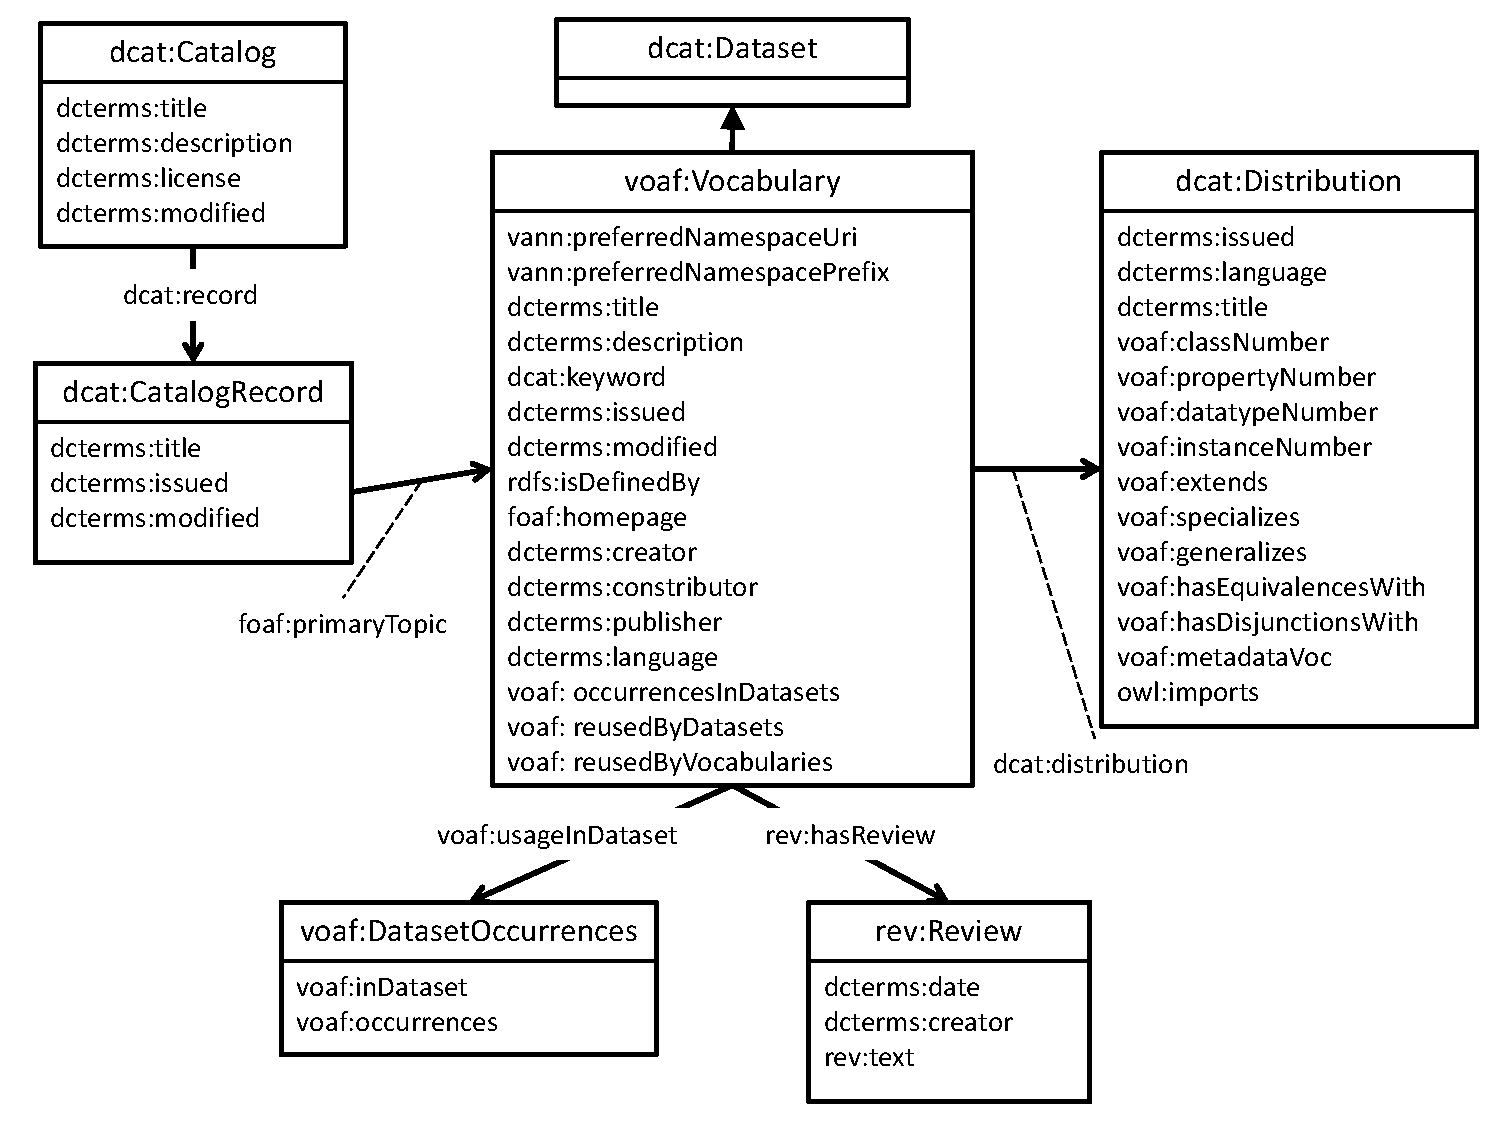
\includegraphics[width=.8\textwidth]{figures/LOV_model.pdf}
\caption{The LOV catalogue RDF schema model, in a UML class diagram representation.}
\label{fig:model}
\end{figure*}

\subsubsection{SPARQL Endpoint}
The LOV SPARQL endpoint\footnote{\url{http://lov.okfn.org/dataset/lov/sparql}} offers a complementary data access method and allows clients to pose complex queries to the server and retrieve direct answers computed over the LOV dataset \cite{sparqles13}. We use the Jena Fuseki triple store to store the N-quads file containing the LOV catalogue and the latest version of each vocabulary. We believe that this is the first service that allows users to query multiple vocabularies at the same time and to detect inter-vocabulary dependencies. 

\subsubsection{LOV Application Program Interfaces and User Interfaces}
LOV APIs give a remote access to the many functions of LOV through a set of RESTful services\footnote{\url{http://lov.okfn.org/dataset/lov/apidoc/}}. The basic design requirements for these APIs is that they should allow applications to get access to the very same information humans do via the User Interfaces. More precisely the APIs give access, through three different services (cf. Figure \ref{fig:apis}), to functions related to:
\begin{itemize} 
			\item Vocabulary terms (classes, properties, datatypes and instances). With these functions, a software application can query the LOV search engine, ask for auto-completion or a suggestion for misspelled terms.
			\item Vocabularies. A client can get access to the current list of vocabularies contained in the LOV catalogue; search for vocabularies, get auto-completion or obtain all details about a vocabulary.
			\item Agents. This provides a software agent with a list of all agent references in the LOV catalogue, a means to search for an agent, get auto-completion and details about an agent.
		\end{itemize}
LOV APIs are a convenient means to access the full functionality and data of LOV. It is particularly appropriate for dynamic Web applications using scripting languages such as JavaScript. The APIs described above have been developed for, and follow the requirements of, Ontology Design and Data Publication tools. 


\begin{figure}[!htb]
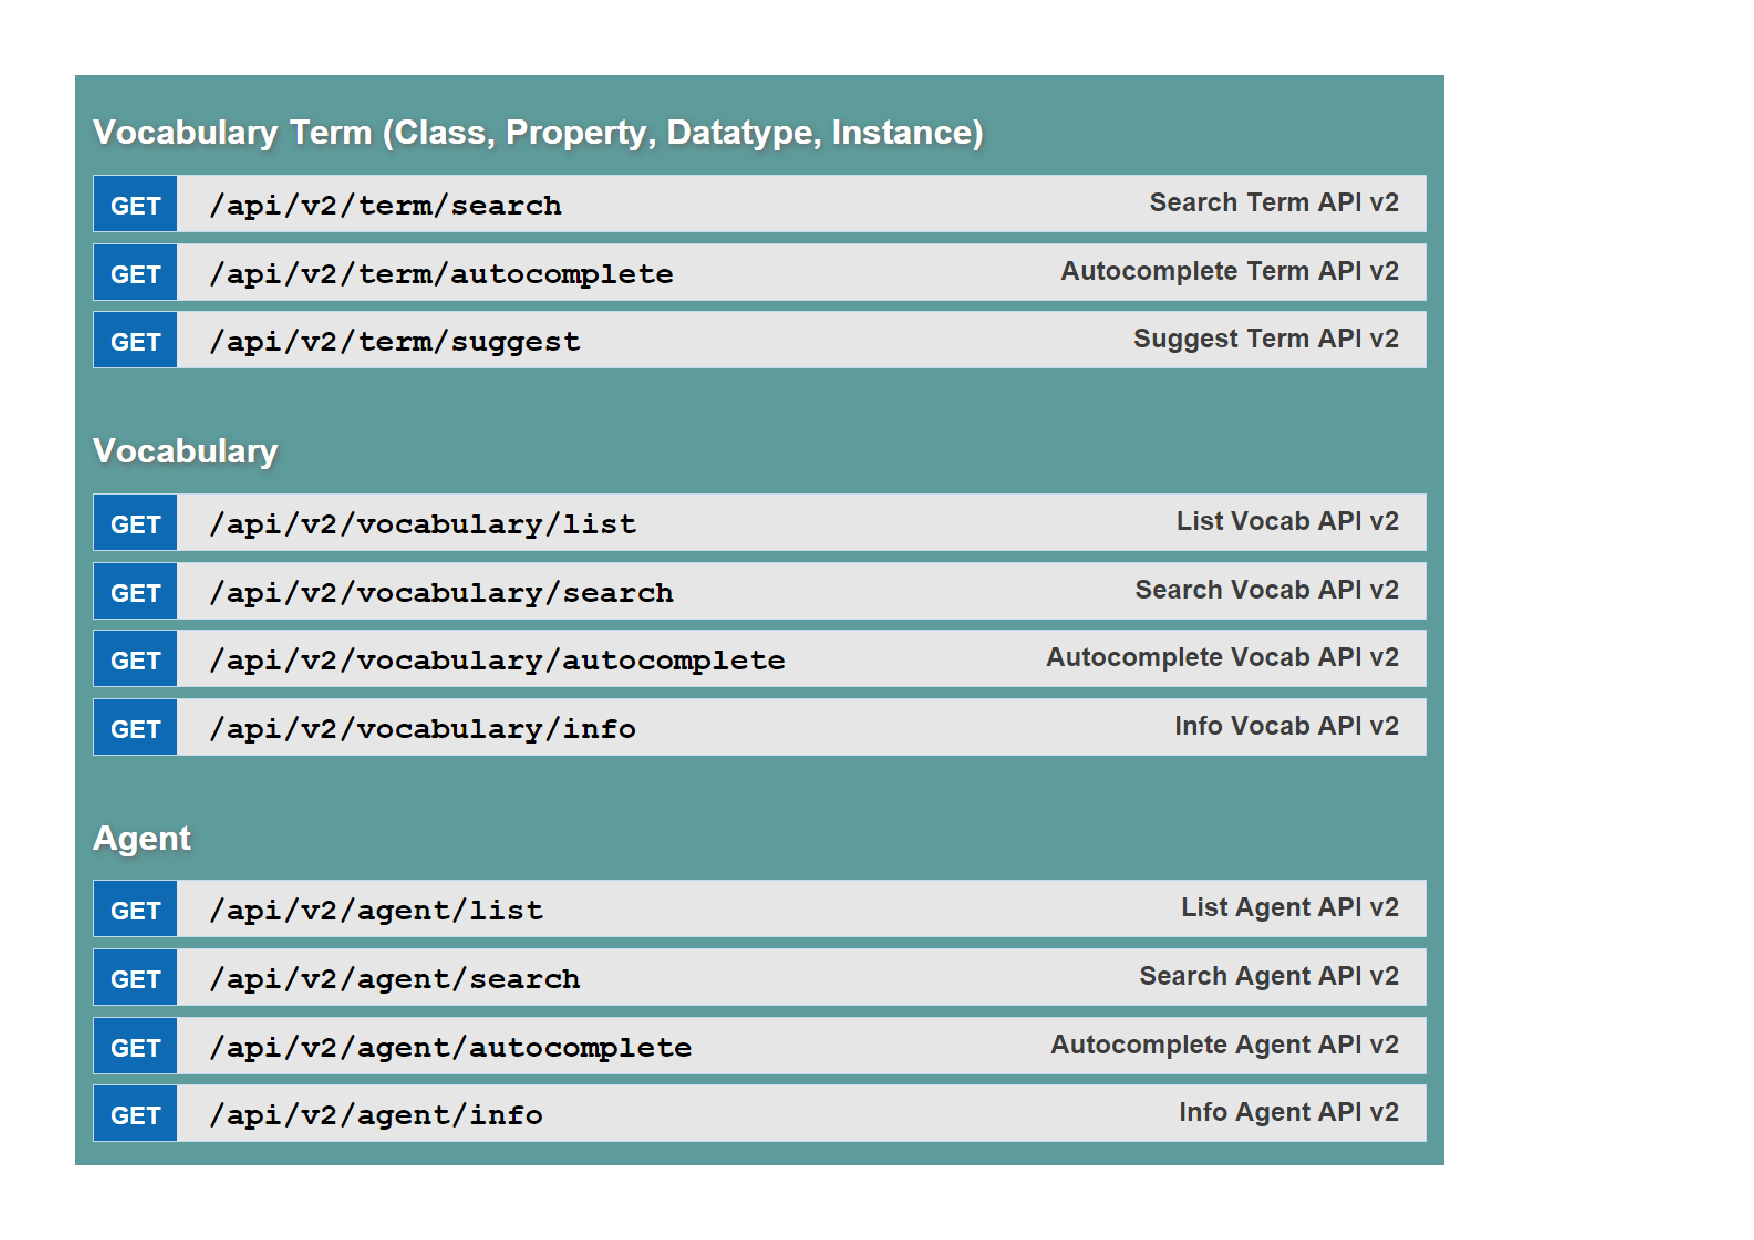
\includegraphics[trim={1cm 1cm 1cm 2cm},width=1.2\textwidth]{figures/apis.pdf}
\caption{List of APIs to access LOV data.}
\label{fig:apis}
\end{figure}

The LOV Website offers intuitive navigation within the vocabularies catalogue. It allows users to explore vocabularies, vocabulary terms, agents and languages, and to see the connections between these entities. For instance, a user can use the agent search to look for experts in \emph{geography} and \emph{geometry} domains\footnote{\url{http://lov.okfn.org/dataset/lov/agents?&tag=Geography,Geometry}}. We use the d3\footnote{\url{http://d3js.org/}} JavaScript library~\cite{d3js} to display charts and make the navigation more interactive; for example, we use the star graph representation to display incoming and outgoing links between vocabularies (cf. Figure \ref{fig:graphVocab}). 


\begin{figure}[ht!b]
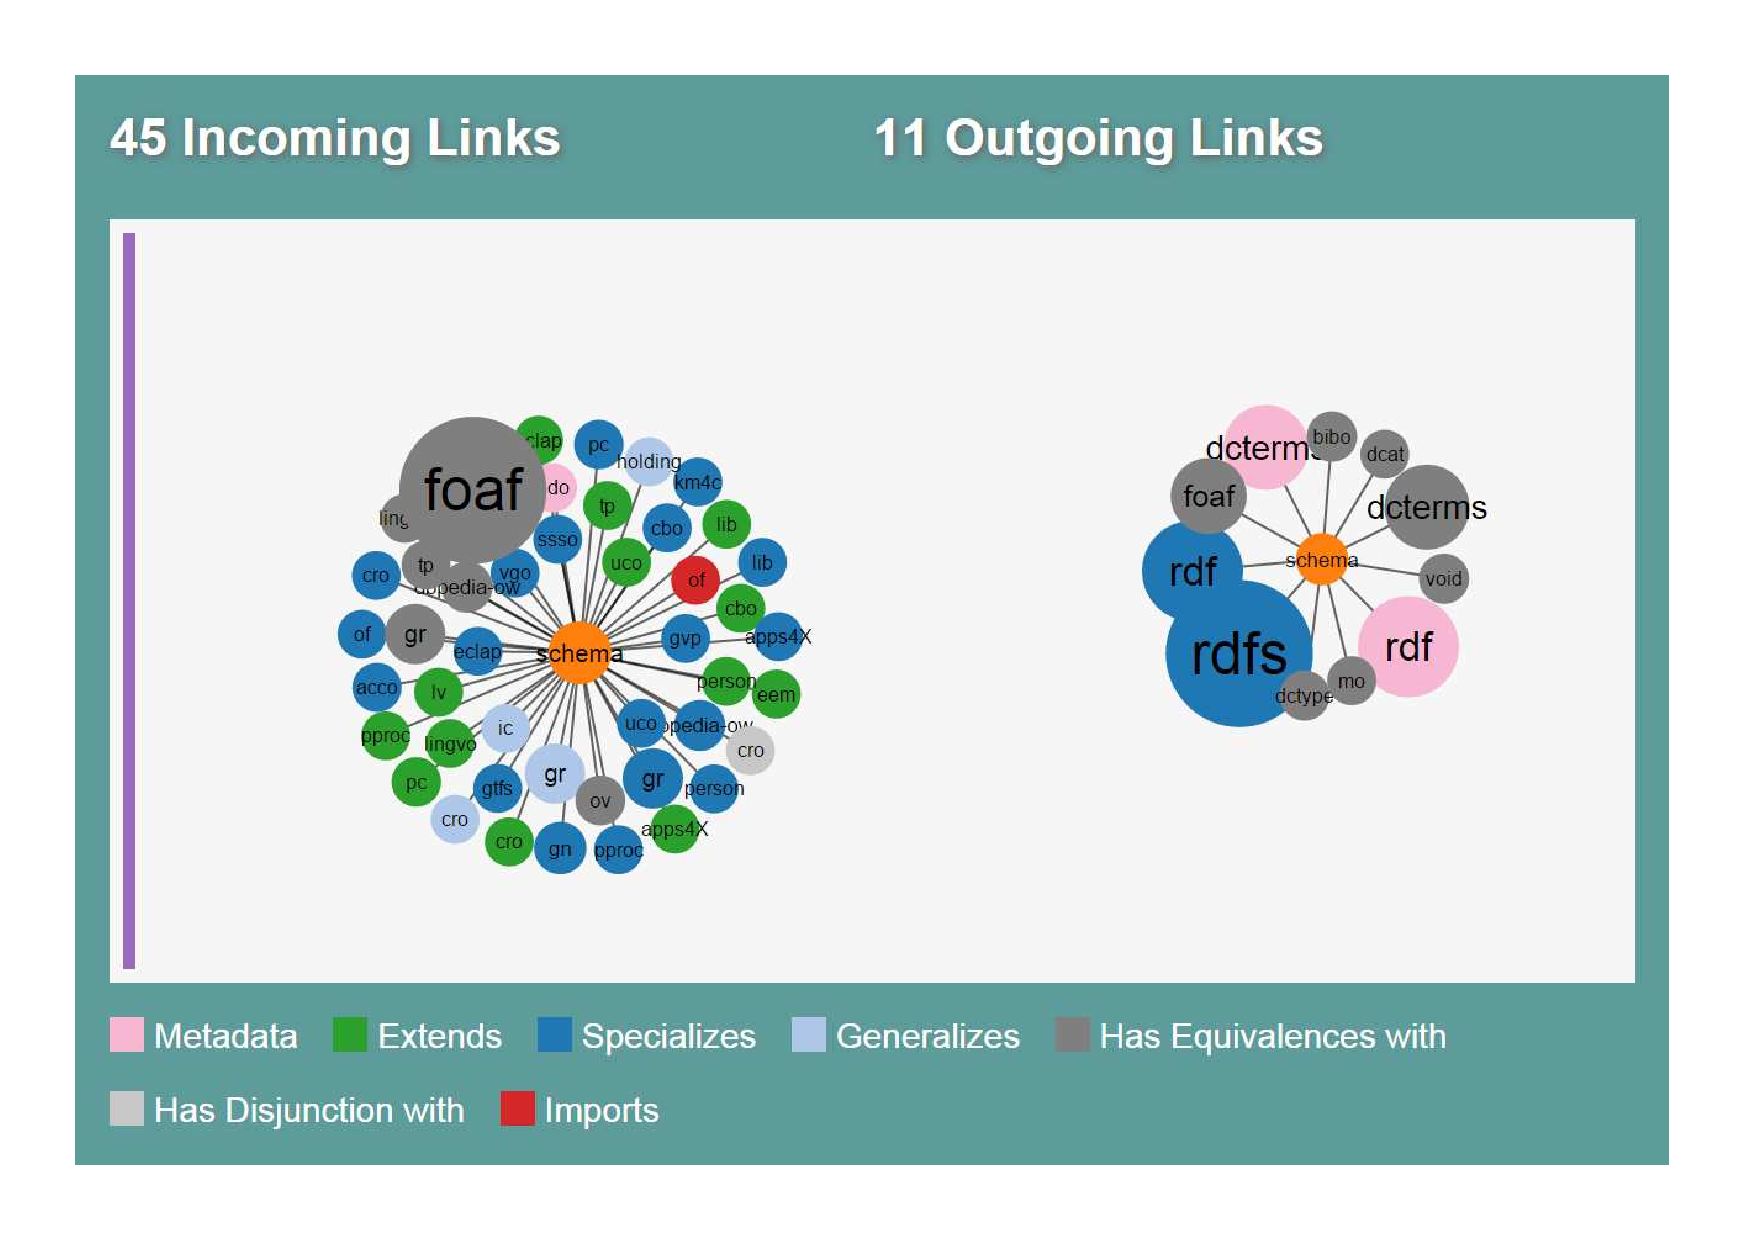
\includegraphics[trim={1cm 1cm 1cm 1cm},width=1\textwidth]{figures/graphVocab.pdf}
\caption{A graphical representation of the incoming and outgoing links for the Schema.org vocabulary as displayed in the UI.}
\label{fig:graphVocab}
\end{figure}

\subsection{Data Storage}

To support the features presented above, we make use of specific storage technologies. The LOV catalogue is stored in MongoDB\textregistered, a document-based schema-less data store that scales and allows for dynamic changes in the data schema\footnote{\url{https://www.mongodb.org/}}. We use Jena Fuseki\footnote{\url{https://jena.apache.org/documentation/serving_data/}} to serve the data exported in RDF through the SPARQL protocol. The search feature is supported by Elasticsearch\textregistered, a full text index based on Lucene technology\footnote{\url{https://lucene.apache.org/}}. This storage solution is particularly well adapted to our User Interface technology (Node.js) as it offers RESTful APIs with output in JSON format. Finally we store each vocabulary version file and RDF dumps of LOV catalogue in the environment file system.


%%%Section: LOV Adoption %%%%
%%%%%%%%%%%%%%%%%%%%%%%%%%%%%

\section{LOV Adoption}\label{sec:lovecosystem}
LOV, with its various data access methods, supports the emergence of a rich application ecosystem. Below we list some tools using our system as part of their service and project.
 
\subsection{Derived tools and applications}

In \cite{ontomaton12}, Maguire \emph{et al.} use the LOV search API to implement OntoMaton\footnote{\url{https://github.com/ISA-tools/OntoMaton}}, a widget for using ontology lookup and tagging within the Google spreadsheets collaborative environment. 

YASGUI (Yet Another SPARQL Query GUI)\footnote{\url{http://legacy.yasgui.org/}} is a client-side JavaScript SPARQL query editor that uses the LOV API for property and class auto-completion together with prefix.cc\footnote{\url{http://prefix.cc}} for namespace prefix auto-completion \cite{yasgui}. YASGUI is itself reused by LOV for its SPARQL Endpoint User Interface.

Data2Ontology maps data objects and properties to ontology classes and predicates available in the LOV catalogue. Data2Ontology is part of the  Datalift\footnote{\url{http://datalift.org/}} platform \cite{scharffe_2012}, a framework for ``lifting'' raw data into RDF. The Data2Ontology module takes as input ``raw RDF'', straightforward conversion of legacy format to RDF, with the goal of helping data publishers in selecting vocabulary terms that could be used to better represent their data.


OntoWiki\footnote{\url{http://ontowiki.net/}} facilitates the visual presentation of a knowledge base as an information map, with different views on instance data~\cite{auer2006ontowiki}. It enables intuitive authoring of semantic content, with an inline editing mode for editing RDF content, similar to WYSIWIG for text documents. OntoWiki offers a vocabulary selection feature based on LOV.

Furthermore, we can mention the Prot{\'e}g{\'e}LOV\footnote{\url{http://labs.mondeca.com/protolov/}}, a plug-in for the Prot{\'e}g{\'e} editor tool \cite{prolov2015} that aims at improving the development of lightweight ontologies by reusing existing vocabularies at a low fine grained level. The tool searches for a term in LOV via APIs and provides three actions if the term exists : 
\begin{inparaenum}[1)] 
 \item to replace the selected term in the current ontology, 
 \item to add the {\small\texttt{rdfs:subClassOf}} axiom and 
 \item to add the {\small\texttt{owl:equivalentClass}}.
\end{inparaenum}



\subsection{Using LOV as a Research platform}

LOV has served as the object of studies in~\cite{poveda2012landscape} where Poveda-Villal\'on \emph{et al.} analysed trends in ontology reuse methods. In addition, the LOV dataset has been used to analyse the occurrence of good and bad practices in vocabularies~\cite{poveda2013detecting}.

Prefixes in the LOV dataset are regularly mapped with namespaces in the prefix.cc service. In~\cite{wasabi13}, the authors perform alignments of Qnames of vocabularies in both services and provide different solutions to handle clashes and disagreements between preferred namespaces. Both LOV and prefix.cc provide associations between prefixes and namespaces but follow a different logic. The prefix.cc service supports polysemy and synonymy, and has a very loose control on its crowd-sourced information. In contrast, LOV has a much more strict policy forbidding polysemy and synonymy ensuring that each vocabulary in the LOV database is uniquely identified by a unique prefix identification allowing the usage of prefixes in various LOV publication URIs. 

The LOV query log covering the period between 2012-01-06 and 2014-04-16 has been used in \cite{butt2014} to build a benchmark suite for ontology search and ranking. The CBRBench\footnote{\url{https://zenodo.org/record/11121}} benchmark uses eight ranking models of resources in ontologies and compares the results  with ontology engineers' results. Our vocabulary term ranking method relies on and extends the outcome of this work.


In \cite{janowicz2014five}, the authors provide a 5 star rating for RDF vocabulary publication to boost interoperability, query federation and better interpretation of data on the Web similar to the 5 stars rating for Linked Open Data. Based on LOV's  best practices criteria, all vocabularies must be 5 stars using this ranking and must provide further quality attributes imposed by LOV to facilitate vocabulary reuse.


RDFUnit\footnote{\url{https://github.com/AKSW/RDFUnit}} is a test-driven data debugging framework for the Web of Data. In~\cite{rdfunit}, the authors provide an automatic test case for all available schema registered with LOV. Vocabularies are used to encode semantics to domain specific knowledge to check the quality of data.

Finally, Governatori et al.~\cite{governatori2014} analyse the current use of licenses in vocabularies on the Web based on the LOV catalogue in order to propose a framework to detect incompatibilities between datasets and vocabularies.


%%%%%%%%%%%%%%%%%%%%%%%%%%%%%%%
%%%%%Section: Related Work %%%%
%%%%%%%%%%%%%%%%%%%%%%%%%%%%%%%

\section{Related Work}
\label{sec:related}
Reusing vocabularies requires searching for terms in existing specialised vocabulary catalogues or search engines on the Web. While we refer the reader to~\cite{AquinJoWS12} for a systematic survey of ontology repositories, below we list some existing catalogues relevant for finding vocabularies:  

\begin{itemize}
 \item \textit{Catalogues of generic vocabularies/schemas} similar to LOV catalogue. Example of catalogues falling in this category are vocab.org\footnote{\url{http://vocab.org/}}, ontologi.es\footnote{\url{http://ontologi.es/}}, JoinUp Semantic Assets or the Open Metadata Registry. Most of those repositories are not regularly updated and are created/owned by the institutions using the service.
 \item \textit{Catalogues of ontologies for a specific domain} such as biomedicine with the BioPortal \cite{bioportal11}, geospatial ontologies with SOCoP+OOR\footnote{\url{https://ontohub.org/socop}}, Marine Metadata Interoperability and the SWEET \cite{sweet05} ontologies\footnote{\url{http://sweet.jpl.nasa.gov//}}. The SWEET ontologies include several thousand terms, spanning a broad extent of Earth system science and related concepts (such as data characteristics), with the search tool to aid finding science data resources. 
 \item \textit{Catalogues of ontology Design Patterns (ODP)} focus on reusable patterns in ontology engineering \cite{presutti08}. The submitted patterns are small pieces of vocabularies that can further be integrated or linked with other vocabularies. ODP does not provide a search function for specific terms as is the case with some of these other catalogues. 
 
 \item \textit{Search Engines of ontology terms}. Among ontology search engines, we can cite: Swoogle~\cite{finin2005swoogle}, Watson~\cite{Sabou07}, FalconS~\cite{cheng2008falcons} and Vocab.cc~\cite{vocabcc2013}. These search engines crawl for data schema from RDF documents on the Web. They offer filtering based on ontology type (Class, Property) and a ranking based on the popularity. They don't look for ontology relations nor do they check if the definition of the ontology is available (usually known as dereferenciation). While in Swoogle the ranking score is displayed, Watson shows the language of the resource and the size. However, none of these services provide any relationship between the related ontologies, or any domain classification of the vocabularies. Table \ref{tab:lovfeatures} presents a summary of key features of LOV with respect to Swoogle, Watson, Falcons and Vocab.cc.
 \item \textit{Datasets and Vocabularies statistics}. In this category we can mention LODStats \cite{demter-2012-ekaw} and the vocabularies derived from the LOD Cloud.  LODStats makes a bridge between datasets and vocabularies gathering up to 32 different statistical criteria based on a statement-stream-based approach for RDF datasets in Datahub\footnote{\url{http://datahub.io/}}. LODStats maintains a comprehensive statistics on vocabularies terms (i.e. classes, properties) defined and used in a dataset. Schmachtenberg et al.~\cite{max2014} present a survey based on a large-scale Linked Data crawl from March 2014 to analyse the differences in best practices adoption across different application domains. Their results concerning the most used vocabularies (e.g., \texttt{foaf}, \texttt{dcterms}, \texttt{skos}, etc.) and the adoption of well-known vocabularies are inline with the findings of this paper.
\end{itemize}


While most of the related work focuses on automatic techniques to gather as many ontologies as possible, LOV focuses on maintaining a high quality collection of vocabularies that data publishers can reuse to describe their own data. To ensure the high quality of LOV data, we set up some stringent requirements for vocabularies to be inserted (cf. Section \ref{sssec:vocabInsert}) such as the fact that a vocabulary URI must be dereferenceable. These kinds of requirements are not always taken into account in the aforementioned work: for instance, the authors in~\cite{max2014} define the notion of partly dereferenceable for vocabularies. As a consequence, anyone using a vocabulary referenced in LOV is ensured to get access to the vocabulary metadata but most importantly to its formal definition and preservation by accessing to various versions. 


 \begin{table*}[!htb]
 \scriptsize
\centering{
\begin{tabular}{|l|l|l|l|l|l|}
\hline
 \textbf{Feature}	& Swoogle & Watson & Falcons & Vocab.cc & LOV 			 \\ \hline
Listing ontologies	   & Yes & Yes & Yes & Yes & Yes \\ \hline
Ontology discovery method   & Automatic & Automatic & Automatic & Automatic & Automatic/Manual \\ \hline
Scope & SWDs & SWDs & Concepts & vocab terms & Vocabularies \\ \hline
Ranking	& LOD metric & LOD metric & LOD metric &  BTC corpus & \\ 
&&&&+ label's property type	& LOD/LOV metric \\ \hline
Domain filtering & No & No & No & No & Yes \\ \hline
Comments and review 	& No & Yes & No & No & Curators	\\ \hline
Web service access & Yes & Yes & Yes & Yes & Yes		\\ \hline
SPARQL endpoint	& No & No & No & No & Yes		\\ \hline
Read/Write	& Read & Read/Write & Read & Read & Read  	\\ \hline
Ontology directory & No & No & No & Yes & Yes \\ \hline
Application platform & No & No & No & N/A & Yes \\ \hline
Storage & Cache & N/A & N/A &  API & Dump/endpoint \\ \hline
Interaction with contributors & No &  N/A & No & No & Yes \\ \hline
Version tracking & No & No & No & No & Yes \\ \hline
Inter-vocab. relationship visualization & No & No & No & No & Yes \\ \hline
		 
		 \hline

\end{tabular}
\caption{Comparison of LOV with respect to Swoogle, Watson, Falcons and Vocab.cc; adapted from the framework presented by d'Aquin and Noy \cite{AquinJoWS12}. SWD stands for Semantic Web Document. }
\label{tab:lovfeatures}
}
\end{table*}

As part of our system evaluation we have compared the list of vocabularies in LOV with the ones in external services (LODStats and the empirical survey of Schmachtenberg et al.~\cite{max2014}) so as to understand the discrepancy.

 
LODStats contains 2,940 vocabularies extracted from datasets listed in Datahub.io. This list contains in fact a large number (2,596) of invalid vocabulary URIs and resource URIs that do not refer to a vocabulary (e.g. {\footnotesize\url{http://data.kingcounty.gov/resource/d665-vvmd/}} or {\footnotesize\url{http://lod2.eu/view}}). The domain ``http://dati.opendataground.it'' contains 962 Resource URIs which are instances and not vocabularies. As a result, only 344 candidate URIs in LODStats are comparable with LOV vocabularies. Out of those 344 URIs, 73 (21.22\%) are covered by LOV. We randomly chose 20 vocabularies not already present in LOV for assessment. None of the randomly chosen vocabularies met LOV requirements and 8 different categories of errors were detected: 
\begin{inparaenum}[1)]
\item Failed to determine the triples content type,
\item  Not found exception, 
\item 403 forbidden, 
\item Unknown host exception, 
\item  Peer not authenticated,
\item 504 gateway,
\item Bad URI and
\item  Unqualified typed nodes are not allowed. 
\end{inparaenum}

Recently, an updated comprehensive empirical survey of Linked Data conformance has been presented by Schmachtenberg et al.~\cite{max2014}. Their survey is based on a large-scale Linked Data crawl from March 2014 to analyse the differences of best practices adoption in different domains. Their results concerning the most used accessible vocabularies and the adoption of well-known vocabularies are inline with the findings of this paper. However, comparing the vocabularies in the LOD cloud with the LOV catalogue needs some alignments. From the 638 mentioned by Schmachtenberg et al., we removed invalid URIs such as domain names such as ``umbel.org''. Additionally we removed misspelled URIs and incomplete URIs. As a result, 270 candidate URIs (42.31\%) can be compared with LOV vocabularies. Based on this analysis, we found that 102 vocabularies in the LOD cloud are already in the LOV catalogue, representing 38\% of the 270 candidates. The general difference of our work with the one presented by Schmachtenberg et al. is that our approach applies strict criteria to include a vocabulary while their approach is dataset driven.


%%%%%%%%%%%%%%%%%%%%%%%%%%%%%%%
%%%%%Section: DISCUSSION %%%%%%
%%%%%%%%%%%%%%%%%%%%%%%%%%%%%%%
\section{Discussion}\label{sec:discussion}
Whilst providing access to high quality vocabularies, LOV system presents several limitations. As described in the last section, LOV system could benefit from an automatic discovery process to suggest vocabulary candidates. We could for instance extract vocabularies from the latest version of the Billion Triple Challenge or the Web Data Commons\footnote{\url{http://webdatacommons.org/}} dataset. Manual curation is a critical activity to ensure the high quality of the LOV catalogue but also represents a limitation. At the moment we have been able to recruit new curators as the catalogue is growing. The version 3 of LOV system automates most of the processes and analyses but there are still some assessment and support activities that only a human can perform.

Currently, LOV's scope focuses on vocabularies for the description of RDF data and does not include any \emph{Value Vocabularies} such as SKOS thesauri. By making the code of LOV system open source, we encourage anyone to set up an instance of the system to target such artifacts. 

LOV relies on external projects such as LODStats to get the valuable information of vocabulary usage in published datasets. At the moment, the popularity information coming from LODStats does not take into account the most recent interest in publishing RDF data using markup language (e.g. \texttt{schema.org}). As a consequence, the popularity measure is incomplete and does not represent all possible use of a vocabulary. In future work we intend to extract those information from the latest datasets versions of the Billion Triple Challenge and the Web Data Commons.
 

From the study of LOV as a dynamic ecosystem we can draw two main lessons learned: the need for more multilingual vocabularies on the Web and the importance of long term preservation of vocabularies. 

Labels are the main entry point to a vocabulary and their associated language is the key. Only 15\% of LOV vocabularies make use of more than one language. Multilingualism is important at least for two reasons: 
\begin{inparaenum}[1)] 
	\item the most obvious one is allowing users to search, query and navigate vocabularies in their native language; and
	\item translation is a process through which the quality of a vocabulary can only improve. Looking at a vocabulary through the eyes of other languages and identifying the difficulties of translation helps to better outline the initial concepts and if necessary refine or revise them. 
\end{inparaenum} 
Hence multilingualism and translation should be native, built-in features of any vocabulary construction, not a marginal task. 

Currently there is no solution for long-term vocabulary preservation on the Web~\cite{Baker2013HLT}. This is a particularly important problem in a distributed and uncontrolled environment where any individual can create and publish a vocabulary. Third parties can reuse such vocabularies and therefore create a dependency on the original vocabulary availability as it retains the semantics of the data. This issue weakens the Semantic Web foundations. 


%%%%%%%%%%%%%%%%%%%%%%%%%%%%
%%% Section: Conclusion %%%%
%%%%%%%%%%%%%%%%%%%%%%%%%%%%

\section{Conclusions and Future work}
\label{sec:conclusion}

In this system report we presented an overview of the Linked Open Vocabularies initiative, a high quality catalogue of reusable vocabularies for the description of data on the Web. The importance of this work is motivated by the difficulty that data publishers have in determining which vocabularies to use to describe their data. The key innovations described in this article include: 
\begin{inparaenum}[1)] 
	\item the availability of a high quality dataset of vocabularies available through multiple access methods 
	\item the curation by experts, making explicit  for the first time the relationships between vocabularies and their version history; and
	\item the consideration of property semantics in term search relevance scoring.
\end{inparaenum}

In the future, the LOV initiative could evolve in several ways. First, an area that is still largely unexplored is multi-term vocabulary search. During the ontology design process, it is common to have more than 20 concepts represented using existing vocabularies or a new one in case there is no corresponding artifact. While we are able to search for relevant terms in LOV it is still the responsibility of the ontology designer to understand the complex relationships between all these terms and come up with a coherent ontology. We could use the network of vocabularies defined in LOV to suggest not only a list of terms but graphs to represent several concepts together. 

Second, we would like to provide more vocabulary based services such as vocabulary matching to help authors add more relationships to other vocabularies. Vocabulary checking is another service the community is asking for. We could integrate useful applications directly into LOV, such as Vapour\footnote{\url{http://validator.linkeddata.org/vapour}}, RDF Triple-Checker\footnote{\url{http://graphite.ecs.soton.ac.uk/checker/}} and OOPS!\footnote{\url{http://oops.linkeddata.es/}}. 

Another research direction is SPARQL query extension and rewriting based on Linked Vocabularies. Using the inter-vocabulary relationships we could transform a query to use the same semantics (same vocabulary terms) as the data source(s) being queried.

Finally, we plan to provide a user study and publish the results on the different usage of LOV by end users. In addition, we plan to include the vocabularies from LODStats and LOD Cloud that are suitable for inclusion in the LOV catalogue.

The adoption and integration of the LOV catalogue in applications for vocabulary engineering, reuse and data quality are significant.
LOV has a central role in vocabulary life-cycle on the Web of data as highlighted by the W3C\footnote{\url{http://www.w3.org/2013/data/}}: \textit{``The success of LOV as a central information point about vocabularies is symptomatic of a need, for an authoritative reference point to aid the encoding and publication of data''}.

%%%%%%%%%%%%%%%%%%%%%%
%%% Section: ACK %%%%%
%%%%%%%%%%%%%%%%%%%%%%

\section*{Acknowledgments}
This work has been partially supported by the French National Research Agency (ANR) within the Datalift Project, under grant number ANR-10-CORD-009; the Spanish project BabelData (TIN2010-17550) and Fujitsu Laboratories Limited. The Linked Open Vocabularies initiative is graciously hosted by the Open Knowledge Foundation. We would like to thank all the members of LOV community and all the editors and publishers of vocabularies who trust in LOV catalogue. A special thank to Phil Archer, Julia Bosque Gil and Jodi Schneider for their valuable feedback and comments on this paper.

\bibliographystyle{plain}
\bibliography{lov}
\end{document}
